\documentclass[conference]{IEEEtran}
\IEEEoverridecommandlockouts
\usepackage{amsmath,amssymb,amsfonts}
\usepackage{graphicx}
\usepackage{url}
\usepackage[hidelinks]{hyperref}
\usepackage{orcidlink}
\usepackage{xcolor}

\begin{document}

\title{Fourier Features Overcome the Spectral Bias of Physics-Informed Networks: A Minimal, Controlled Demonstration}

\author{\IEEEauthorblockN{Felix Schaller \orcidlink{0000-0002-3218-3214} \href{https://orcid.org/0000-0002-3218-3214}{0000-0002-3218-3214}}
\IEEEauthorblockA{Independent Researcher\\
Dubai, UAE / Munich, Germany\\
Email: \href{mailto:inquiry@felixschaller.com}{inquiry@felixschaller.com}}
\thanks{Preprint. Companion to the benchmark preprint ``Where Fourier Beats Convolution.'' Code, demo and animation: \url{https://github.com/freshNfunky/Fourier-Physics-Informed-NN} and \url{https://huggingface.co/spaces/freshNfunky/fourier-vs-plain-pinn}.}}

\maketitle

\begin{abstract}
Physics-informed neural networks (PINNs) inherit the spectral bias of their coordinate-network backbone: the high-frequency content of a solution converges exponentially slower than the low-frequency content. We give a minimal, fully reproducible demonstration that a Fourier-feature input encoding removes this bias inside a physics-informed loss. On a balanced multi-scale problem, recovering $u(x)$ from the residual of a first-order ordinary differential equation, a plain coordinate network stalls at about half the amplitude of a mode $m=15$ across five thousand training steps, while a Fourier-feature network at matched budget reaches it within a few hundred steps. The problem is balanced by construction, a first-derivative operator with a $1/m$ target amplitude, so that both source modes weigh equally in the residual and the observed effect is spectral bias rather than loss imbalance. We also name the concrete risk that a naive extrapolation misses: the residual differentiates the network, multiplying each Fourier mode by $|k|^{\mathrm{order}}$, which makes the feature bandwidth a sharp knob when scaling to real, higher-order operators. This note isolates the mechanism behind the Fourier advantage documented in the accompanying operator-learning benchmark, and frames the compressible, shock-resolving case as the next study.
\end{abstract}

\begin{IEEEkeywords}
Physics-informed neural networks, spectral bias, Fourier features, coordinate networks, scientific machine learning
\end{IEEEkeywords}

\section{Introduction}
A physics-informed neural network represents the solution of a differential equation as a continuous function $u_\theta(x,t)$ and trains it on the residual of the governing equation, evaluated by automatic differentiation, with few or no solution labels in the interior \cite{raissi2019pinn}. The backbone is a coordinate multilayer perceptron: its input is a point in space-time, its output the field value there. That choice is what makes the residual differentiable pointwise, and it is also the source of a well-documented failure. Plain coordinate networks exhibit a spectral bias, learning low frequencies first and high frequencies exponentially slower \cite{rahaman2019}, so multi-scale and stiff solutions converge poorly.

The remedy that the representation-learning literature proposes is a Fourier-feature encoding of the input coordinate \cite{tancik2020}, and the neural-tangent-kernel analysis of Fourier-feature networks makes the mechanism precise: the features reshape the kernel spectrum so that all target frequencies are learned at comparable rates \cite{wang2021eigenvector}. This underlies a broader thesis, that Fourier ideas are underrated in scientific machine learning. Our aim here is narrow and honest: to isolate the effect in a physics-informed loss on the cleanest possible problem, to report it as a convergence-rate phenomenon rather than a representational wall, and to name the specific risk that scaling the idea will face.

\section{Setup}
\subsection{Backbones}
We compare two periodic coordinate networks at matched parameter budget. The \emph{plain} network encodes the coordinate with the base frequency only, $[\sin 2\pi x,\ \cos 2\pi x]$; the \emph{Fourier-feature} network encodes it across many frequencies, $[\sin 2\pi k x,\ \cos 2\pi k x]_{k=1}^{K}$. Both feed a four-layer $\tanh$ network. A plain $\tanh$ network is not frequency-limited, since its nonlinearity synthesizes harmonics, so any difference we observe is a difference in convergence rate, not in expressible functions.

\subsection{A balanced multi-scale problem}
To isolate spectral bias we deliberately avoid a second-order (Poisson-type) operator, whose $k^2$ scaling would make the source dominated by the high mode and turn the experiment into a loss-weighting artifact. Instead we recover $u(x)$ from the residual of a first-order equation,
\begin{equation}
u'(x) = g(x), \qquad x \in [0,1)\ \text{periodic}, \qquad u(0)=0,
\end{equation}
for the multi-scale target
\begin{equation}
u^\star(x) = \sin(2\pi x) + \tfrac{1}{m}\,\sin(2\pi m x), \qquad m = 15 .
\end{equation}
Then $g(x)=u^{\star\prime}(x)=2\pi\cos(2\pi x)+2\pi\cos(2\pi m x)$: because a first-derivative operator scales as $k$, the $1/m$ amplitude cancels the $m$ and both source modes carry the \emph{same} weight $2\pi$ in the residual. The loss is therefore balanced across scales, and the only question left is whether each network reaches the high mode. Training minimizes the mean squared residual over collocation points sampled fresh each step, plus a single anchor term fixing the additive constant. Both networks use identical optimizer, schedule, and step budget.

\section{Result}
Fig.~\ref{fig:pinn} reports the outcome. Both backbones fit the dominant low mode; they split on the high mode $m=15$. The plain network's error at that mode stalls at about $0.033$, roughly half of the true amplitude $1/m\approx0.067$, and does not improve over five thousand steps; its final relative $L^2$ error is $0.067$. The Fourier-feature network drives the high-mode error to near zero within a few hundred steps and reaches a relative $L^2$ error of essentially zero at the same budget. The per-wavenumber view is unambiguous: a single tall plain spike at the fine-detail frequency stands against a flat Fourier floor.

\begin{figure}[!t]
\centering
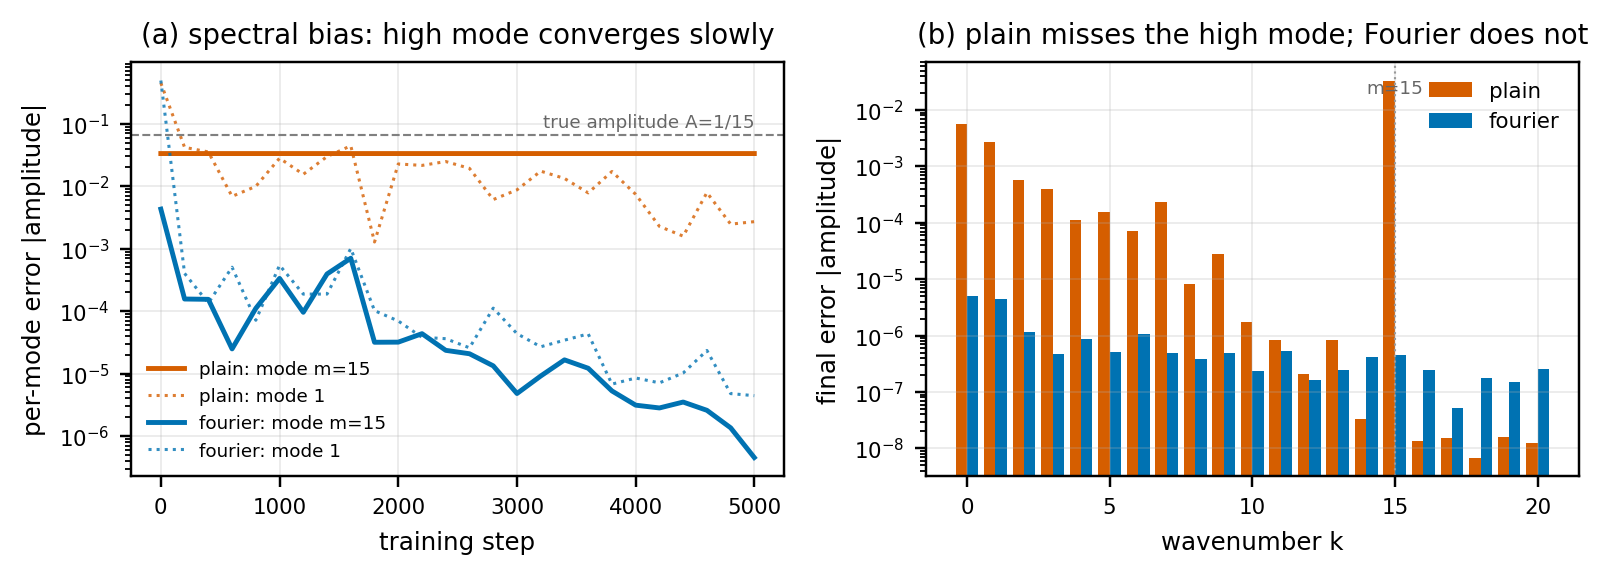
\includegraphics[width=\columnwidth]{figs/pinn_spectral_bias}
\caption{Physics-informed spectral bias. Left: the per-mode error over training; the plain network's high mode ($m=15$) stalls while the Fourier-feature network's decays steadily. Right: the final error per wavenumber, a single tall plain spike at the fine-detail frequency against a flat Fourier floor. Both networks are trained only on the PDE residual, at matched budget.}
\label{fig:pinn}
\end{figure}

\section{Discussion}
The demonstration confirms, inside a physics-informed loss and on a balanced problem, the mechanism that the operator-learning literature attributes to Fourier representations: the advantage is a convergence-rate effect on high frequencies, and the encoding is what unlocks them. It also exposes the risk that a naive extrapolation would miss. The physics residual differentiates the network, up to second order for many partial differential equations, and differentiation multiplies each Fourier mode by $|k|^{\mathrm{order}}$. An over-broad feature bandwidth therefore amplifies high-frequency error inside the residual and can destabilize training. The feature bandwidth is a sharp knob, not a free improvement, and this is precisely why the result does not follow automatically from the data-driven case: the residual changes the game.

Two directions follow. First, the compressible, finite-speed formulation is the physically honest setting for scaling this, because it respects finite propagation rather than the instantaneous global pressure of the incompressible idealization. Second, the same band-resolved and regime-boundary methodology used in the companion operator benchmark should be applied here, adding convergence speed and residual stability as PINN-specific axes, and sweeping the feature bandwidth as the ablation.

\section{Reproducibility}
The problem, both networks, the residual training and the figure are implemented in a few dozen lines of PyTorch and run on a single CPU in under a minute. The exact script and configuration are released with the companion repository.

\begin{thebibliography}{9}
\bibitem{raissi2019pinn} M. Raissi, P. Perdikaris, and G. E. Karniadakis, ``Physics-Informed Neural Networks,'' \emph{Journal of Computational Physics}, 2019.
\bibitem{rahaman2019} N. Rahaman et al., ``On the Spectral Bias of Neural Networks,'' in \emph{ICML}, 2019.
\bibitem{tancik2020} M. Tancik et al., ``Fourier Features Let Networks Learn High Frequency Functions in Low Dimensional Domains,'' in \emph{NeurIPS}, 2020.
\bibitem{wang2021eigenvector} S. Wang, H. Wang, and P. Perdikaris, ``On the eigenvector bias of Fourier feature networks: From regression to solving multi-scale PDEs with physics-informed neural networks,'' \emph{Computer Methods in Applied Mechanics and Engineering}, 2021.
\end{thebibliography}

\end{document}
